\section{Errors and Correction}
\label{sec:error_detection}
As mentioned in the beginning of this chapter, there are many issues that the physical layer does not concern itself with. One of those is errors in the transmission of data. The physical layer is responsible for the transmission of bits, but it does not guarantee that those bits will arrive at their destination without errors.

There are many different types of errors and approaches to mitigating/correcting them! Too many to cover in this reader, even!

Most protocols in the data-link layer discard the frame when errors are detected. However, some wireless protocols attempt to correct the frame instead of discarding it.

\subsection{Types of Errors}
There are three primary types of errors that can occur during data transmission. \textbf{Interference} refers to unpredictable changes that can alter the shape of the signal, often caused by external factors such as electromagnetic noise or physical obstructions. 

A \textbf{single-bit error} occurs when only one bit of a given data unit has changed from its original value, typically representing the most common and least severe form of data corruption. 

In contrast, a \textbf{burst error} is more serious, involving two or more bits in the data unit that have changed, which can significantly impact data integrity and is often harder to detect and correct.

\subsection{Error Detection}
Error detection is AWESOME! But also very math heavy. The basic idea is to add some extra bits to the data being transmitted, which can be used to check if the data has been corrupted during transmission.

\subsubsection{Block Coding}
Block coding is the foundation of most error detection schemes. The concept is beautifully simple: take your original data (called the \textbf{dataword}) and systematically add extra bits (called \textbf{redundancy bits}) to create a longer \textbf{codeword}.

\begin{figure}[h]
    \centering
    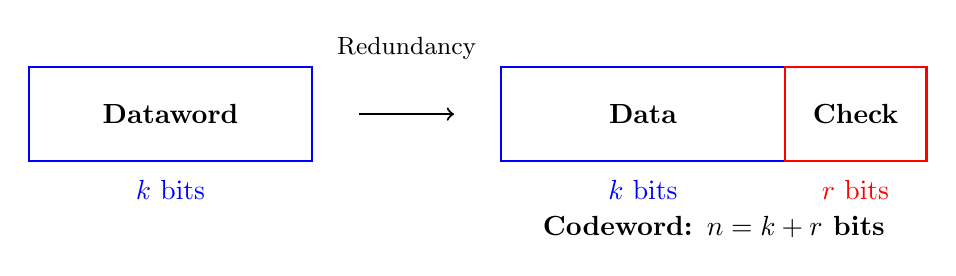
\begin{tikzpicture}[scale=1.2]
        % Dataword
        \draw[thick, blue] (0,1) rectangle (3,2);
        \node at (1.5,1.5) {\textbf{Dataword}};
        \node[blue] at (1.5,0.7) {$k$ bits};
        
        % Arrow
        \draw[->, thick] (3.5,1.5) -- (4.5,1.5);
        \node at (4,2.2) {\small Redundancy};
        
        % Codeword
        \draw[thick, blue] (5,1) rectangle (8,2);
        \draw[thick, red] (8,1) rectangle (9.5,2);
        \node at (6.5,1.5) {\textbf{Data}};
        \node at (8.75,1.5) {\textbf{Check}};
        \node[blue] at (6.5,0.7) {$k$ bits};
        \node[red] at (8.75,0.7) {$r$ bits};
        \node at (7.25,0.3) {\textbf{Codeword: $n = k + r$ bits}};
    \end{tikzpicture}
    \caption{Block coding adds redundancy bits to create error-detectable codewords}
    \label{fig:block_coding}
\end{figure}

Not all possible $n$-bit patterns are valid codewords - only specific combinations are allowed. When errors occur during transmission, the received pattern might not match any valid codeword, alerting us to corruption.

\subsubsection{Parity Bits: The Simplest Error Detection}
Parity\footnote{A number's parity is the property of being even or odd. In the context of error detection, it refers to the number of 1s in a binary representation.} checking is the most basic form of error detection. We add a single bit that makes the total number of 1s in the codeword either even (\textbf{even parity}) or odd (\textbf{odd parity}).

Let's see how even parity works with a 4-bit dataword:

\begin{table}[h]
\centering
\begin{tabular}{|c|c|c|c|c|c|}
\hline
\multicolumn{4}{|c|}{Dataword} & Parity & \multicolumn{1}{c|}{Total 1s} \\
\hline
$d_3$ & $d_2$ & $d_1$ & $d_0$ & $p$ & Count \\
\hline
0 & 0 & 0 & 0 & 0 & 0 (even) \\
0 & 0 & 0 & 1 & 1 & 2 (even) \\
0 & 0 & 1 & 0 & 1 & 2 (even) \\
0 & 0 & 1 & 1 & 0 & 2 (even) \\
0 & 1 & 0 & 0 & 1 & 2 (even) \\
\ldots & \ldots & \ldots & \ldots & \ldots & \ldots \\
\hline
\end{tabular}
\caption{Even parity ensures the total number of 1s is always even}
\label{tab:parity_example}
\end{table}

\textbf{Detection process:}
\begin{enumerate}
    \item Sender calculates parity bit and transmits dataword + parity
    \item Receiver counts all 1s in the received codeword
    \item If count is odd (for even parity), an error is detected
    \item If count is even, assume no error (though this isn't guaranteed!)
\end{enumerate}

\paragraph{Limitations of Simple Parity}
Simple parity can detect any \textbf{odd number} of bit errors (1, 3, 5, \ldots) but cannot detect \textbf{even numbers} of errors (2, 4, 6, \ldots). For example:

\begin{align*}
\text{Original:} \quad &1011\mathbf{0} \quad \text{(even parity, 3 ones total)}\\
\text{2-bit error:} \quad &1\mathbf{1}\mathbf{0}1\mathbf{0} \quad \text{(still even parity, 3 ones total)}
\end{align*}

The receiver would not detect this corruption! Simple parity operates on the principle of counting 1s, and when an even number of bits flip, the parity remains unchanged. In our example, the original codeword 10110 has three 1s (odd count), so with even parity we add a 0 to make it 101100 (four 1s total - even). After the 2-bit error occurs, 111100 still has four 1s (even count), so the parity check passes despite the data being corrupted.

This fundamental limitation occurs because parity checking uses modulo-2 arithmetic (XOR operations). When we flip an even number of bits, the XOR result remains the same:
\[
\text{bit}_1 \oplus \text{bit}_2 \oplus \ldots \oplus \text{bit}_n = \text{same result if even number of bits change}
\]

In fact, simple parity has a \textbf{50\% probability} of missing errors when multiple bits are corrupted - not much better than random guessing for multi-bit errors!

\paragraph{Two-Dimensional Parity}
To improve error detection, we can arrange data in a rectangular grid and add parity bits for both rows and columns:

\begin{figure}[h]
    \centering
    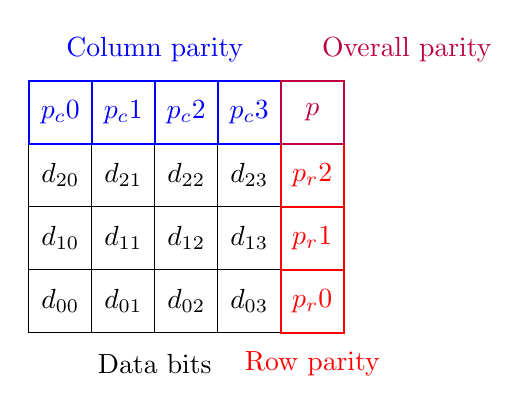
\begin{tikzpicture}[scale=0.8]
        % Data grid
        \foreach \i in {0,1,2} {
            \foreach \j in {0,1,2,3} {
                \draw (\j,\i) rectangle (\j+1,\i+1);
                \node at (\j+0.5,\i+0.5) {$d_{\i\j}$};
            }
        }
        
        % Row parity
        \foreach \i in {0,1,2} {
            \draw[red, thick] (4,\i) rectangle (5,\i+1);
            \node[red] at (4.5,\i+0.5) {$p_r\i$};
        }
        
        % Column parity
        \foreach \j in {0,1,2,3} {
            \draw[blue, thick] (\j,3) rectangle (\j+1,4);
            \node[blue] at (\j+0.5,3.5) {$p_c\j$};
        }
        
        \draw[purple, thick] (4,3) rectangle (5,4);
        \node[purple] at (4.5,3.5) {$p$};
        
        % Labels
        \node at (2,-0.5) {Data bits};
        \node[red] at (4.5,-0.5) {Row parity};
        \node[blue] at (2,4.5) {Column parity};
        \node[purple] at (6,4.5) {Overall parity};
    \end{tikzpicture}
    \caption{Two-dimensional parity can detect and sometimes correct single-bit errors}
    \label{fig:2d_parity}
\end{figure}

Two-dimensional parity can:
\begin{itemize}
    \item Detect most patterns of 2-bit and 3-bit errors
    \item Locate and even correct single-bit errors
    \item Still fail for certain 4-bit error patterns
\end{itemize}

\subsubsection{Cyclic Redundancy Check (CRC)}
While parity bits are simple, they're not very powerful. For better error detection, we turn to Cyclic Redundancy Check (CRC) - this is actually being used in real-life networks.

CRC is based on \textbf{polynomial arithmetic} over finite fields. Don't panic! The math is elegant once you understand the pattern.

\paragraph{The Big Idea}
Think of your data as coefficients of a polynomial. For example, the bits \texttt{1101} represent:
\[
1 \cdot x^3 + 1 \cdot x^2 + 0 \cdot x^1 + 1 \cdot x^0 = x^3 + x^2 + 1
\]

CRC works by:
\begin{enumerate}
    \item Treating data as a polynomial $M(x)$
    \item Choosing a \textbf{generator polynomial} $G(x)$
    \item Computing the remainder when $x^r \cdot M(x)$ is divided by $G(x)$
    \item Appending this remainder as the CRC bits
\end{enumerate}

\begin{importantblock}
    If no errors occur, the received codeword will be perfectly divisible by $G(x)$. If division leaves a remainder, we know errors have occurred.
\end{importantblock}

\begin{noteblock}
    CRC-32 (used in Ethernet and many other protocols) has a 32-bit check sequence and can detect virtually all error patterns in practice. The probability of an undetected error is approximately $2^{-32} \approx 2.3 \times 10^{-10}$ - incredibly small!
\end{noteblock}

TODO: CRC calculation details\ldots